% Template for Cogsci submission with R Markdown

% Stuff changed from original Markdown PLOS Template
\documentclass[10pt, letterpaper]{article}

\usepackage{cogsci}


\title{TODO}


\author{{\large \bf Veronica Boyce (vboyce@stanford.edu)} \\ Department of Psychology, \\Stanford University \And {\large \bf Ben (TODO email) } Department of Psychology, \\Stanford University \AND {\large \bf Alvin (TODO email)} \\ TODO affiliation, Stanford University \And {\large \bf Michael C. Frank (mcfrank@stanford.edu)} \\ Department of Psychology, \\ Stanford University}


\begin{document}

\maketitle

\begin{abstract}
TODO abstract

\textbf{Keywords:}
TODO keywords
\end{abstract}

\section{Introduction}\label{introduction}

Conversation pacts and partner specificity are often studied by looking
at how they are constructed; an additional perspective comes from how
opaque or interpretable they are to outsiders who weren't part of the
pact

By measuring opaqueness in different conditions related to how the pacts
were formed or what the language looks like, can get another perspective
on the process of pact formation

An empirical test of partner - specificity

Prior work to cover Summary of ref games \& claims around them
(\textbf{hawkins2020b?}) (\textbf{clark1986?}) etc

The side-participant / overhearer etc literature
(\textbf{wilkes-gibbs1992?}), \& lit search for more

Judy's work Visual resemblance and interaction history jointly constrain
pictorial meaning (\textbf{hawkinsb?})

possible could also mention other times when naive comprehender has been
used to better understand iteractive dialogues?

``Why use models'' -- can frame opaqueness as semantic distance between
utterance and referent -- models are an explicit test of this! ``Naive
comprehender'' / ``matcher''

\subsection{ALvin gets to write computational intro
here}\label{alvin-gets-to-write-computational-intro-here}

Do we also want to motivate this from a computational angle?
(i.e.~trying to add pragmatics to models) TODO not me

\subsection{back to Veronica}\label{back-to-veronica}

Key question: What properties of conversational pacts and the process of
their formation make them more or less easy for an outsider to
understand?

We use both human experiments and models to assess when and why
expressions are opaque or understandable to outside observers.

\section{Task Setup}\label{task-setup}

\subsection{Materials}\label{materials}

We draw on the corpus of reference game transcripts and results from
(\textbf{boyce2024?}). There were all 6 round iterated reference games
using the same 12 target images, but varied in how large the groups were
(2-6 participants per group) and how ``thick'' the communication channel
between group members was. For our human experiments, we sample
different subsets of this corpus in different experiments. Within the
samples, we avoided showing participants descriptions that had swear
words or crude or sexual language. We use the entire corpus for our
computational modelling component.

\subsection{Experimental procedure}\label{experimental-procedure}

We recruited participants from Prolific (TODO criteria). Participants
were directed to the experiment, where it was explained that previously,
other participants had described these shapes to one another. They would
see a series of transcripts from the prior game, and their task was the
guess what the intended target was. On each trial participants saw the
full transcript from that trial, containing all the chat messages marked
by whether they were from the speaker or a listener (TODO confirm the
language used), except for lines that (\textbf{boyce2024?}) had marked
as not having any referential content. Participants selected the image
they thought was the target from the tableau of 12. Participants
received feedback on whether they were right or wrong on each trial.
Except when the specific viewing order was part of the experimental
manipulation, we randomized the order of trials, subject to the
constraint that the same target could not repeat on adjacent trials.\\
The task was implemented in jsPsych. We paid participants \$10 an hour
plus a bonus of 5 cents per correct response.

\begin{CodeChunk}
\begin{figure}[t!]

{\centering 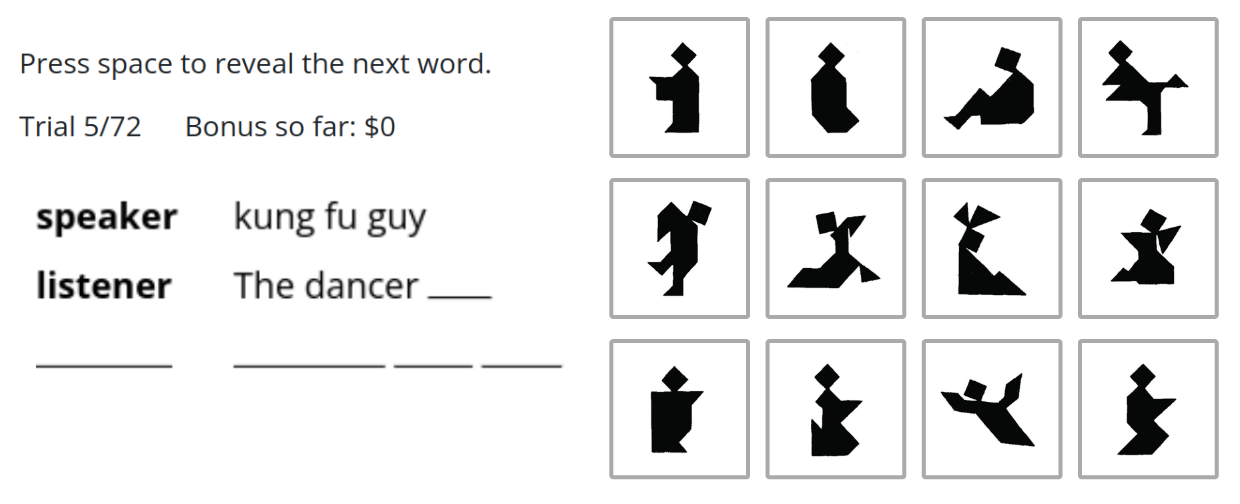
\includegraphics[width=1\linewidth]{matcher_diagram} 

}

\caption[Experimental Setup and Procedure.TODO REPLACE \label{game}]{Experimental Setup and Procedure.TODO REPLACE \label{game}}\label{fig:interface}
\end{figure}
\end{CodeChunk}

\subsection{Computational models that Ben gets to
write}\label{computational-models-that-ben-gets-to-write}

Computational methods TODO V doesn't know how to write this QUESTION: do
we focus on mlp pre- or post- calibration?

\section{Calibration expt that Alvin gets to
write}\label{calibration-expt-that-alvin-gets-to-write}

\begin{CodeChunk}
\begin{figure}[t]

{\centering 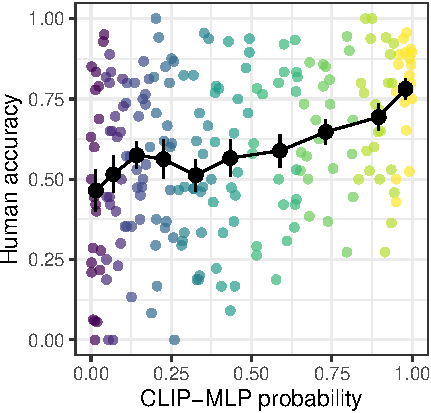
\includegraphics[width=0.7\linewidth]{figs/fig-calibration-1} 

}

\caption[Correlation between human and CLIP-MLP accuracy across deciles of CLIP-MLP accuracy]{Correlation between human and CLIP-MLP accuracy across deciles of CLIP-MLP accuracy. Colored points are individual descriptions, black line is the boostrapped mean and 95\% CI across descriptions for each decile. \label{calibration}}\label{fig:fig-calibration}
\end{figure}
\end{CodeChunk}

TODO methods

pre-reg at \url{https://osf.io/6pv5e}

modeling approach and selection

how well can models proxy humans? are there differences?

tg-matcher 3 (calibration) 61 participants, 64 items each, from a pool
of 217 transcripts spanning the models full accuracy range

\section{Experiment 2}\label{experiment-2}

As a starting point for examining what makes referential expressions
more or less opaque, we had people read the descriptions from the
beginnings and ends of games. The idea of reduction and
partner-specificity would suggest that the conventionalized, later round
utterances would rely on the history of the game that naive matchers
were not privy to, and thus that late round utterances would be more
opaque and difficult to understand. On the other hand, describers gained
practice over repetitions, so later round utterances might be better at
clearly communicating the most visually salient features.

We included descriptions from games of different sizes and communication
thicknesses. In terms of group conditions, based on the patterns of
cross-game similarity in (\textbf{boyce2024?}), we thought that smaller
and thicker games were more likely to rapidly develop ideosyncratic
conventions that would be more opaque than the less ideosyncratic
conventions from larger groups with thinner communication channels.

\subsection{Methods}\label{methods}

\subsubsection{Experiment 2a}\label{experiment-2a}

To establish a baseline of how well naive matchers could understand
descriptions without context, we ran a 2x2 within subjects experiment.
We drew the target transcripts from 2 and 6 player games from Experiment
1 of (\textbf{boyce2024?}) and from the first and last (sixth) blocks of
these games. These games had medium thick communication channels. We
recruited 60 participants who each saw 60 trials (15 in each of the 4
conditions). Overall, participants saw 774 transcripts from 40 games.
This experiment was pre-registered at \url{https://osf.io/k45dr}.

\subsubsection{Experiment 2b}\label{experiment-2b}

After observing limited condition differences in experiment 2a, we ran a
second study drawing from the more extreme communication channel
thicknesses of Experiment 3 in (\textbf{boyce2024?}). Here, we used a
2x2x2 within subjects design, drawing our transcripts from the thick and
thin, 2 and 6 person, 1st and 6th block utterances. In the thin
condition, original matchers could only contribute to the chat by
sending one of 4 emojis; as the emojis did not have referential content,
we did not include them in the transcripts shown to naive matchers. For
experiment 2b, we recruited 60 participants who each saw 64 trials (8 in
each of the 8conditions). Overall, participants saw 2392 transcripts
from 163 games. This experiment was pre-registered at
\url{https://osf.io/rdp5k}.

\begin{CodeChunk}
\begin{figure}[t]

{\centering 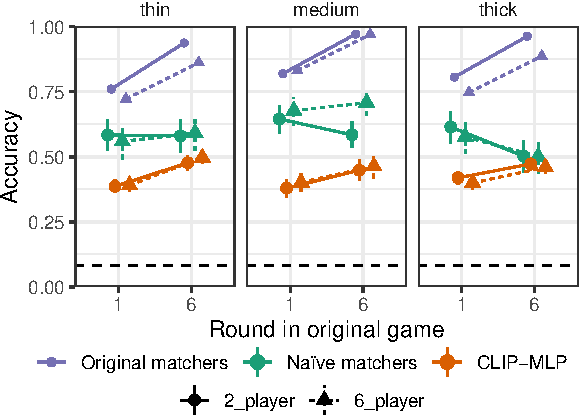
\includegraphics[width=0.9\linewidth]{figs/fig-condition-1} 

}

\caption[Accuracies for naive humans and the CLIP-MLP model for Experiment 2]{Accuracies for naive humans and the CLIP-MLP model for Experiment 2. Point estimates and 95\% CrI are predictions from the fixed effects of logistic and beta regressions. Bootstrapped mean accuracy from the original matchers is included as a ceiling, and random chance as a baseline. \label{expt2-condition}}\label{fig:fig-condition}
\end{figure}
\end{CodeChunk}

\begin{CodeChunk}
\begin{figure}[t]

{\centering 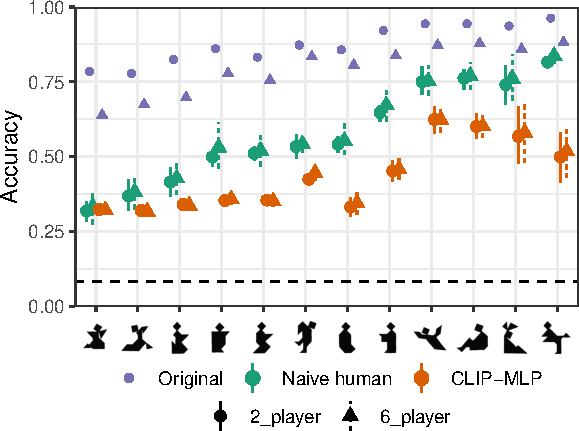
\includegraphics[width=0.9\linewidth]{figs/fig-2-1} 

}

\caption[Accuracies for naive humans and the CLIP-MLP model for Experiment 2, split out by target image]{Accuracies for naive humans and the CLIP-MLP model for Experiment 2, split out by target image. Point estimates and 95\% CI are predictions from the fixed effects and by-tangram random effects of logistic and beta regressions, bootstrapped across conditions. Bootstrapped mean accuracy from the original matchers is included as a ceiling, and random chance as a baseline. \label{expt2-tangram}}\label{fig:fig-2}
\end{figure}
\end{CodeChunk}

\subsection{Results}\label{results}

Our primary outcome was how accurate naive matchers would be at
selecting the correct target, and how much this would vary depending on
what game and what round the description came from.

\subsubsection{Experiment 2a}\label{experiment-2a-1}

For Experiment 2a, we ran a mixed effects logistic model of naive
matcher accuracy: correct\(\sim\) group\_size \(\times\) round~+
trial\_order~+ (group\_size \(\times\) round\textbar correct\_tangram)~+
(group\_size \(\times\) round~+ trial\_order\textbar workerid). Overall,
naive matchers were right more often than not, which was far above the
1/12 expected by random chance3 (OR: 1.93 {[}1.05, 3.62{]}. As seen in
Figure \ref{expt2-condition} middle panel, there were not large effects
of condition. Participants tended to be less accurate at descriptions
from the last round (OR of last round: 0.77 {[}0.53, 1.1{]}). There was
not a clear effect of transcripts from 6-player games (OR: 1.15 {[}0.89,
1.47{]}), but there was an interaction between round and group size (OR:
1.49 {[}1.06, 2.1{]}). Later transcripts from larger games were easier
to understand, but later transcripts from smaller games were easier to
understand. Much of the variation in accuracy was instead driven by
variation in the target images (OR of standard deviation of image
distribution: 2.66 {[}1.88, 4.52{]}. Some images were much easier to
identify as the target than others (Figure \ref{expt2-tangram}.

\subsubsection{Experiment 2b}\label{experiment-2b-1}

For Experiment 2b we ran a similar mixed effects logistic model,
consider the effects of group size, thickness, and round and their
interactions. Overall, naive matchers were above 50\% accuracy (OR: 1.81
{[}1.06, 3.08{]}). Similar to experiment 2a, there were not substantial
effects of condition. Last round descriptions had slightly lower
accuracy (OR of last round: 0.64 {[}0.47, 0.85{]}), but there was an
interaction with thickness, where thin, last round were less opaque (OR:
1.55 {[}1.02, 2.33{]}).

Again some of the uncertainty in estimating the fixed effects was driven
by the strong effects of target image (OR of SD of images: 2.25 {[}1.67,
3.59{]}).

\subsubsection{Additional Predictors}\label{additional-predictors}

As additional post-hoc predictors, we also examined the predictive value
of the accuracy of the original matchers from (\textbf{boyce2024?}) and
the the length of the description from the original describer. In both
experiments, original accuracy was predictive of naive matcher accuracy
(Expt 2a OR: 3.38 {[}2.46, 4.7{]}, Expt 2b OR: 2.17 {[}1.7, 2.77{]}).
The log number of words in the description was not predictive in
Experiment 2a (OR: 1.05 {[}0.94, 1.17{]}), but longer descriptions were
slightly beneficial in Experiment 2b (OR: 1.1 {[}1.01, 1.2{]}).

\subsection{Model results}\label{model-results}

As a computational comparison, we looked at the CLIP-MLP model's
performance on the same descriptions. We used the probability the model
assigned as a measure of the model's accuracy, and fit a beta regression
on the descriptions from Experiment 2: correct\(\sim\) group\_size
\(\times\) thickness \(\times\) round~+ (group\_size \(\times\)
thickness \(\times\) round\textbar correct\_tangram). The CLIP-MLP model
was far above chance, but had lower accuracy than the human participants
(OR: stats\_text(acc\_mod\_mlp, 1) .

None of the fixed effects in the model were significant, and there was
wide uncertainty for all of them. There is substantial by-tangram
variation 1.58 {[}1.31, 2.15{]} and substantial by-tangram variation in
the effect of later round 1.56 {[}1.29, 2.09{]}.

As additional predictors, we checked the effect of original matcher
accuracy and the length of the description. MLP-CLIP had higher accuracy
when original matcher accuracy was higher (OR: 1.5 {[}1.33, 1.69{]}),
and the model did better on shorter descriptions (OR for log words: 0.85
{[}0.82, 0.9{]}). Long descriptions may be further from the model's
training distribution of image captions.

\subsubsection{Interim Summary}\label{interim-summary}

Overall, naive human matchers were fairly accurate overall, but less
accurate than matchers in the original game. Perhaps surprisingly, this
level of accuracy was fairly consistent across descriptions from
different times in the game and different game conditions. The largest
source of variability was from the target images; while there was some
variabiliity in accuracy by images for the original matchers, there was
substantially more variability for naive matchers.

\section{Experiment 3}\label{experiment-3}

In Experiment 2, we saw that naive matchers could understand the
descriptions fairly well, but had lower accuracy than the matchers in
the original games. There are several differences between these two,
including getting descriptions from a consistent group, getting
descriptions in order, and being a present participant during the game.
In Experiment 3, we focus on the role of context and group-specific
interaction history to tease apart some of these differences.

\subsection{Methods}\label{methods-1}

Following CITE ROBERT AND JUDY, we compared naive matchers in ``yoked''
and ``shuffled'' conditions. In the ``yoked'' condition, naive matchers
saw all the descriptions from a single game in the order they originally
occurred. In the ``shuffled'' condition, naive matchers saw all the
descriptions from a single game in a randomized order.

Because some descriptions are already pretty understandable in
isolation, we wanted to focus on the role of context in games that
showed strong group-specificity. We hand-picked 10 games from
(\textbf{boyce2024?}) on the basis of high original matcher accuracy,
strong reduction in the length of utterances, and the use of
idiosyncratic or non-modal referring expressions. Thus, the referring
expressions were very understandable to groups who created them, but
likely to be opaque out of context.

We recruited 196 participants (99 in the yoked condition and 97 in
shuffled) who each saw all 72 trials of 1 of the 10 games. This
experiment was pre-registered at \url{https://osf.io/zqwp5}.
Participants read the transcripts in a modified self-paced reading
procedure where they uncovered the text word by word (revealed words
stayed visible); only after uncovering the entire transcript could
participants select an image. We do not analyse the word-by-word reading
data here.

\begin{CodeChunk}
\begin{figure}[t]

{\centering 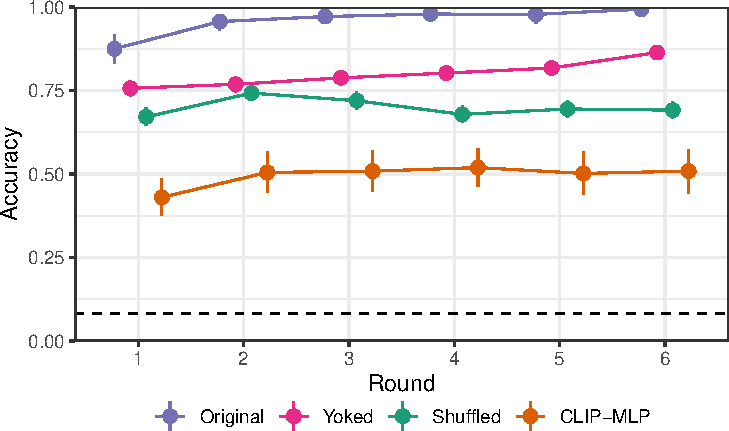
\includegraphics[width=0.9\linewidth]{figs/fig-yoked-1} 

}

\caption[Accuracies for Experiment 3]{Accuracies for Experiment 3. Error bars are bootstrapped 95\% CIs. TODO not using predictions because those fuzz out round to round differences. \label{yoked}}\label{fig:fig-yoked}
\end{figure}
\end{CodeChunk}

\subsection{Results}\label{results-1}

Our primary question of interest was how much having the conversation
history would help make later round descriptions more understandable to
participants in the yoked condition.

We compared accuracy across the yoked and shuffled conditions with a
logistic regression: correct\(\sim\) orig\_repNum \(\times\) condition~+
matcher\_trialNum~+ (1\textbar gameId)~+ (1\textbar correct\_tangram)~+
(1\textbar workerid). The descriptions were more transparent when they
were presented in a yoked order (OR: 2.2 {[}1.63, 3{]}, Figure
\ref{yoked}). In the shuffled condition, there was no main effect of
round number (OR for one round later: 0.99 {[}0.95, 1.02{]}), but there
was a marginal interaction where the benefit of the yoked condition
decreased for later rounds (OR for one round later: 0.94 {[}0.89, 1{]}).
This was offset by matchers in both conditions improving at the task
over time (OR for one trial later in matcher viewing order: 1.02
{[}1.02, 1.02{]}). In the yoked condition round and trial number were
aligned, so an improvement over time could be either from matcher
practice or from descriptions being easier to understand. In the
shuffled condition, matcher practice effects did not line up with
position in the original game.

Comparing with the performance of the original matchers, we can separate
out the benefits of seeing the descriptions in order versus being a live
participant: correct\(\sim\) orig\_repNum \(\times\) order~+
orig\_repNum \(\times\) setting~+ matcher\_trialNum~+
(1\textbar gameId)~+ (1\textbar correct\_tangram)~+
(1\textbar workerid). There is a benefit to seeing the items in order
(OR: 2.24 {[}1.63, 3.04{]}) and a larger benefit to being a participant
during the game in real-time (OR: 4.35 {[}2.77, 6.89{]}). The benefit of
seeing the items in order wanes in later blocks (OR: 0.94 {[}0.89,
1{]}), but the benefit of being in the real-time game does not (OR: 1.06
{[}0.95, 1.18{]}). In all cases, there is a baseline improvement over
trials (OR: 1.02 {[}1.02, 1.02{]}).

The accuracy of the CLIP-MLP model is worse than the shuffled human
results, and does not show change across rounds (OR for one round later:
1.02 {[}0.97, 1.07{]}). The larger difference between naive human and
CLIP-MLP accuracies in Experiment 3 than Experiment 2 could suggest that
even the shuffled ordering still provides useful context that helps
matchers understand the conventions. This history is not available to
the CLIP-MLP model which sees every description as a one-shot task.

QUERY: we could run the model without matcher\_trial\_num which flips
the direction of interactions because it centers later, and also you get
to see the benefit of (matcher) experience purely in terms of the
repNum. I think it's better the way it is, but raising it.

NOTE: not showing model estimates in Figure 5 b/c the fit isn't great,
not sure why\ldots{}

\section{Discussion ?}\label{discussion}

\subsection{Part of discussion that Alvin gets to
write??}\label{part-of-discussion-that-alvin-gets-to-write}

Discussion

Understanding varies much more based on item than on anything else;
potentially due to priors or iconicity of image (? that might be beyond
scope -- how well does this match up with say diversity of descriptions)

Models do pretty well? IDK what our model take away is

Especially when there is strong or idiosyncratic reduction, context
helps

role of context

limitations, incuding out of distribution for models

might want to address language comprehension v inference

\section{References}\label{references}

\setlength{\parindent}{-0.1in} 
\setlength{\leftskip}{0.125in}

\noindent

\bibliographystyle{apacite}


\end{document}
